% !TeX spellcheck = en_GB
% !TeX root = Report.tex
\phantomsection
\addcontentsline{toc}{subsection}{Lecture 3 - Iain Gavin \& Amazon Web Services}
\subsect{Lecture 3 - Iain Gavin \& Amazon Web Services}

Amazon is, without any reasonable doubt, an established company.
Founded by Jeff Bezos in 1994, the company shipped their first book in July 1995~\cite{seattle}.
The company now has three different parallel business interests.
The original retail aspect, the 3$^{rd}$ party selling service via the website and Amazon Web Services (AWS).
AWS powers the other two aspects of the business by providing the infrastructure that enables such excellent customer service but also acts as an accelerator for other businesses by removing the requirement for on-premises IT solutions.
They achieve this by maintaining large sever farms from which computing power can be \emph{rented} to facilitate the IT needs of a company.
They also provide varying degrees of cloud based storage; subject to access latency.

AWS considers a typical split in effort toward a computing heavy buiness venture, with on premises IT solutions, to be $30$\% towards the actual business and $70$\% towards IT overheads. 
Their goal is to flip this distubution by providing the infrastructe. 
One such company that has acceled using AWS is Hailo~\cite{gavin2014ams}.
Launched in $2011$ with investments totalling over \$$80$ million from some well known sources; including Union Square Ventures, Accel Partners and Sir Richard Branson~\cite{hailo}.
The company maintains a smartphone app that links customers with the local taxi services to provide.


\inote{Need to sexify}


\begin{figure}
	\centering
	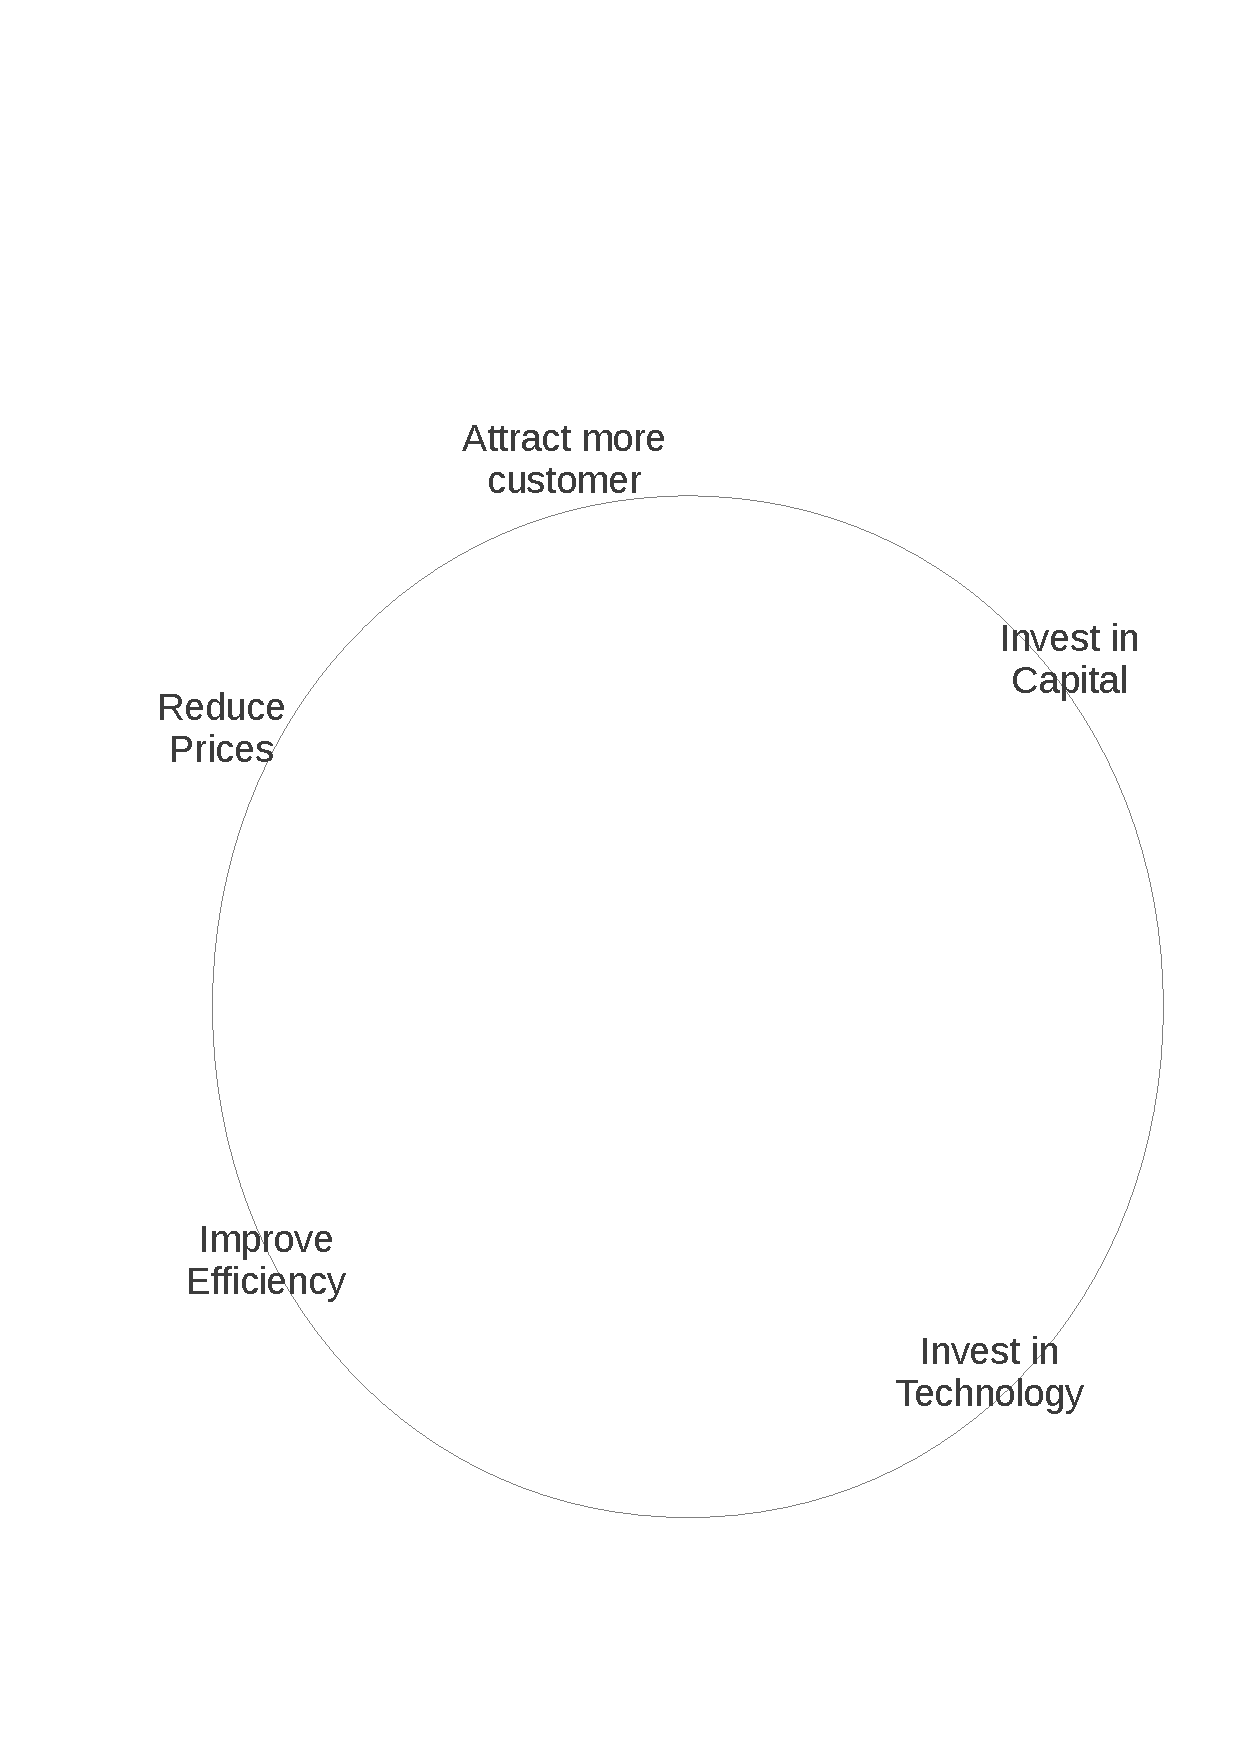
\includegraphics[width=0.5\textwidth]{./Figures/ScaleInnovation.pdf}
	\caption{Scale \& Innovation Drives Down Costs. Taken from~\cite{gavin2014ams}.}
	\label{fig:ScaleInnovation}
\end{figure}

